\documentclass[output=paper,colorlinks,citecolor=brown]{langscibook}
\ChapterDOI{10.5281/zenodo.20611899}
\author{Vincent Renner\orcid{}\affiliation{Université Lumière Lyon 2} and Adam Renwick\orcid{}\affiliation{Université Grenoble-Alpes}}

\title{Inflection dropping in the English-origin verbs of present-day French}

\abstract{Fifty frequent English-origin verbs extracted from a corpus of 100 million French tweets from 2020--2022 were analyzed for uninflectedness in two composite verb forms -- the \emph{passé composé} construction and the periphrastic future construction. It was found that a majority of these verbs show a substantial preference for the nonstandard practice of dropping inflectional marking on the past participle (for the \emph{passé composé}) and the infinitive (for the periphrastic future). This salient feature of written social media discourse is unexpected as it violates a presumably categorical norm but it is not truly exceptional in light of other underreported phenomena of verbal uninflectedness, especially when French is in contact with other languages. It is also suggested that unadapted forms are not only a marked choice flagging foreignness and peripherality, but also, in some cases, markers of in-group membership.}


\IfFileExists{../localcommands.tex}{
   \addbibresource{../localbibliography.bib}
   \usepackage{tabularx,multicol}
\usepackage[hyphens]{url}
\urlstyle{same}

\usepackage{langsci-optional}
\usepackage{langsci-lgr}
\usepackage{langsci-gb4e}

\usepackage{soul}
% \usepackage{booktabs}
% \usepackage{geometry}
\usepackage{multirow}
% \usepackage{makecell} %safely breaks a line inside a table cell
% \usepackage{tablefootnote} %footnotes in table captions
\usepackage{enumerate}
\usepackage{tikz}
\usepackage{array}
\usepackage[shortlabels]{enumitem}

%for having several figures on one line, turning words in 90°angles
% \usepackage{graphicx}
\usepackage{subcaption}

% \usepackage{caption} %for making the caption line longer in concrete cases

% \usepackage{rotating} %rotate a whole page; for large tables

\usepackage{fontspec}
\newfontfamily\charis{Charis SIL} %for being able to use the symbol ‿ and a better command of some of the boldfaced diacritics in 01
\newfontfamily\japanesefont{Noto Serif CJK JP} % for Japanese script
% \usepackage{tipa}

% \usepackage{needspace} %to keep exs on one page

\usepackage{xcolor}

\usepackage{pgfplots}
\pgfplotsset{compat=1.18}

%%%%%   AVMs for 02	%%%%%
\usepackage{langsci-avm}
\avmsetup{switch = ?}


\usepackage{langsci-branding}

   %\newcommand*{\orcid}{}


\makeatletter
\let\thetitle\@title
\let\theauthor\@author
\makeatother

\newcommand{\togglepaper}[1][0]{
   \bibliography{../localbibliography}
   \papernote{\scriptsize\normalfont
     \theauthor.
     \titleTemp.
     To appear in:
     E. Di Tor \& Herr Rausgeberin (ed.).
     Booktitle in localcommands.tex.
     Berlin: Language Science Press. [preliminary page numbering]
   }
   \pagenumbering{roman}
   \setcounter{chapter}{#1}
   \addtocounter{chapter}{-1}
}

\newbool{bookcompile}
\booltrue{bookcompile}
\newcommand{\bookorchapter}[2]{\ifbool{bookcompile}{#1}{#2}}



\renewcommand{\thempfootnote}{\fnsymbol{mpfootnote}} % use * for footnotes in float env

% \newcolumntype{L}[1]{>{\raggedright\arraybackslash}p{#1}} %left-aligned (non-justified) text in tables
% \newcolumntype{R}[1]{>{\raggedleft\arraybackslash}p{#1}} % right-aligned (non-justified) text in tables

\definecolor{customgreen}{RGB}{27,158,119}
\definecolor{custompink}{RGB}{231,42,138}
\definecolor{customblue}{RGB}{117,112,179}
\definecolor{customlightblue}{RGB}{143,170,220}
\definecolor{customdarkblue}{RGB}{68,114,196}
\definecolor{customyellow}{RGB}{225,192,0}
\definecolor{customorange}{RGB}{233,137,21}
\definecolor{customgray}{RGB}{229,229,229}


% Left-aligned indexes
% % \makeatletter
% % \patchcmd{\theindex}{\twocolumn}{\raggedright\twocolumn}{}{}
% % \makeatother

%to make Japanese scripts in the bibliography smaller
\newcommand{\japbib}[1]{{\japanesefont\small #1}}

%%%%%%%%%%%%%%%%%%%	MACROS for 02	%%%%%%%%%%%%%%%%

%%% Formatting	%%%%%

\newcommand{\textex}[1]{\textit{#1}} 		 %for formatting linguistic examples in-text%
%command-shift X

\newcommand{\lxm}[1]{\textsc{#1}}  		%for formatting names of lexemes
%command-option-shift L

%%%%%%%%% Abbreviations	%%%%%%

\newcommand{\featname}[1]{\textsc{#1}}
\newcommand{\featspec}[2]{\featname{#1}:{#2}}
\newcommand{\feat}[2]{\textsc{#1}:{#2}}  				% \feat{FEATURE}{value}  sc's
\newcommand{\featnameonly}[1]{\textsc{#1}} 			% \featnameonly{featurename}  sc's

\newcommand{\pr}{$^{\prime}$}

\newcommand{\Corr}{\textit{Corr}}
\newcommand{\propm}{\textit{pm}}

\newcommand{\PC}{Π$_{C}$}

\newcommand{\PF}{Π$_{F}$}
\newcommand{\PR}{Π$_{R}$}

\newcommand{\lex}{$\mathcal{L}$}

   %% hyphenation points for line breaks
%% Normally, automatic hyphenation in LaTeX is very good
%% If a word is mis-hyphenated, add it to this file
%%
%% add information to TeX file before \begin{document} with:
%% %% hyphenation points for line breaks
%% Normally, automatic hyphenation in LaTeX is very good
%% If a word is mis-hyphenated, add it to this file
%%
%% add information to TeX file before \begin{document} with:
%% %% hyphenation points for line breaks
%% Normally, automatic hyphenation in LaTeX is very good
%% If a word is mis-hyphenated, add it to this file
%%
%% add information to TeX file before \begin{document} with:
%% \include{localhyphenation}
\hyphenation{
    Al-ex-an-der
    Ber-ber
    chan-ges
    cir-cum-stan-ces
    coin-age
    Fraj-zyngier
    ita-liano
    Ja-pa-nese
    Kö-nig
    Krzy-żanowski
    li-te-ra-tur-no-go
    mi-zen-kei
    par-a-digm
    phe-nom-e-non
    ren-tai-shi
    Slo-vene
    Spen-cer
    Stoj-kov
    Ver-bi-ca-re-se
    wide-spread
}

\hyphenation{
    Al-ex-an-der
    Ber-ber
    chan-ges
    cir-cum-stan-ces
    coin-age
    Fraj-zyngier
    ita-liano
    Ja-pa-nese
    Kö-nig
    Krzy-żanowski
    li-te-ra-tur-no-go
    mi-zen-kei
    par-a-digm
    phe-nom-e-non
    ren-tai-shi
    Slo-vene
    Spen-cer
    Stoj-kov
    Ver-bi-ca-re-se
    wide-spread
}

\hyphenation{
    Al-ex-an-der
    Ber-ber
    chan-ges
    cir-cum-stan-ces
    coin-age
    Fraj-zyngier
    ita-liano
    Ja-pa-nese
    Kö-nig
    Krzy-żanowski
    li-te-ra-tur-no-go
    mi-zen-kei
    par-a-digm
    phe-nom-e-non
    ren-tai-shi
    Slo-vene
    Spen-cer
    Stoj-kov
    Ver-bi-ca-re-se
    wide-spread
}

   \boolfalse{bookcompile}
   \togglepaper[23]%%chapternumber
}{}

\begin{document}
\maketitle

\section{Introduction} 

\begin{sloppypar}
The literature on the morphological adaptation of anglicisms\is{anglicism} in present-day \ili{French} has so far largely focused on nouns and adjectives and \citet{saugera2012-english, saugera2012-inflectional} has convincingly argued that the specific classes of items that resist plural inflection marking generally do so in accordance with subrules that originate within the \ili{French} morphological system. Verbs are generally less frequently borrowed than nouns \citep{tadmor2009} and less attention has been paid to verbal anglicisms\is{anglicism} in the literature. Their adaptive behavior is generally appraised as follows: while the adaptation of foreign-origin nouns and adjectives to the \ili{French} inflectional system is variable, that of borrowed verbs is obligatory \citep{anastassiadissymeonidisnikolaou2011, poplack2017} and contact with \ili{English} has had no significant impact on the grammatical core of the language as \ili{French} verbs continue to be conjugated \citep{sauliere2014}. These general statements may, however, need to be partially reevaluated in light of the recent emergence of uninflected \ili{English}-origin verbal forms, as illustrated by the following tweet excerpts, in (\ref{09ex1}--\ref{09ex3}), and news magazine article title, in (\ref{09ex4}):
\end{sloppypar}

\begin{exe}
	\ex \label{09ex1}
	J'ai \ul{crush} sur une meuf avec qui je travaillais.
	\trans ‘I had a crush on a chick I was working with.’ \\
	\hfill (the inflected past participle form \textit{crushé} is expected)
	
	\ex \label{09ex2}
	Je vais \ul{spoil} donc lisez pas le thread si vous êtes pas à jour sur le manga.
	\trans ‘I'm going to spoil things so don't read the thread if you're not up to date on the manga.’ \\
	\hfill (the inflected infinitive form \textit{spoiler} is expected)
	
	\ex \label{09ex3}
	Je viens de \ul{play} cette vidéo en salle de pause à fond.
	\trans ‘I've just played this video in the break room with the volume full on.’ \\
	\hfill (the inflected infinitive form \textit{player} is expected)
	
	\ex \label{09ex4}
	Esclavage : l'Écosse s'apprête-t-elle à ``\ul{cancel}'' son patrimoine historique ?
	\trans ‘Slavery: Is Scotland about to ``cancel" its historical heritage?’
	
	\hfill (Marianne, 22 Dec. 2021)\footnote{\url{https://www.marianne.net/monde/europe/esclavage-lecosse-sapprete-t-elle-a-cancel-son-patrimoine-historique} (last accessed on 13 June 2024)} \\
	\hfill (the inflected infinitive form \textit{canceler} is expected)
\end{exe}

Such occurrences could be brushed aside as individual ungrammatical oddities but their recurring presence in random searches on the social network\is{social media} Twitter\footnote{This research was conducted before \emph{Twitter} became known as \emph{X}, which is why only \emph{Twitter} is used in this chapter.} acted as a spur to take this incipient phenomenon as seriously as it deserves and to attempt to measure the extent to which it is widespread in contemporary written social media discourse\is{social media}, in the broader context of keyboard-to-screen communication (KSC)\is{keyboard-to-screen communication (KSC)} \citep{juckerdurscheid2012}.

The remainder of this chapter is organized as follows: Section \ref{09sec2} describes the different steps taken to obtain a representative sample of 50 frequent \ili{English}-origin verbs in a large corpus of \ili{French} tweets. Section \ref{09sec3} presents the distribution of the inflected and uninflected forms in the \emph{passé composé} and periphrastic future constructions found in the corpus. Section \ref{09sec4} discusses the various findings in the light of other phenomena of verbal uninflectedness, particularly when \ili{French} is in contact with other languages, and concludes.

\section{Methods} \label{09sec2}

Uninflected verbal forms in present-day \ili{French} are hypothesized to be a morphological feature more typical of colloquial discourse and the difficulty of accessing vast corpora of spoken data led to relying on written social media data\is{social media}, which are known to epitomize register hybridity, mixing informal spoken features with more formal written ones, and to exhibit the same heterogeneity and patterns of linguistic change as non-KSC speech\is{keyboard-to-screen communication (KSC)} \citep{tagliamontedenis2008, bohmann2020}. Building an ad hoc corpus from Twitter data was opportunistic as the Academic Research Access API allowed for easy collection of millions of \ili{French} tweets. Starting from the premise that verbal uninflectedness was an exceptional behavior and in order to keep the task of data processing manageable, only two constructions intuitively identified as more likely to contain instances of audible inflection dropping were selected for this exploratory study: the \emph{passé composé} construction, which is formed with the auxiliary verb \emph{avoir} (`to have') followed by a past participle and encodes either primary or secondary past tense \citep{mosegaardhansen2016}, and the periphrastic future construction, which is formed with the auxiliary verb \emph{aller} (`to go') followed by an infinitive and encodes secondary future tense (\citealt{mosegaardhansen2016}). This choice was in part motivated by the fact that several highly frequent verbal inflectional markers are inaudible in \ili{French} (by default, the three singular forms of the present indicative are, for instance, homophonous with the verbal root) and that spelling alone is not a reliable cue for inflectional (non-)marking in written social media discourse\is{social media} (in spontaneous written production, i.e. a situation in which spelling is not controlled, or standardized, it is not possible to determine whether inaudible deviations from the orthographic norm are deliberate, reflect the imposition of time or practical constraints on the act of typing, or indicate defective mastery of the standard written code).

Our corpus was assembled using the TAGS application \citep{hawksey2016} to automate weekly queries for the two target constructions over a 15-month period, from November 2020 to February 2022, in pools of tweets automatically tagged as being in \ili{French} (without any geographical specification) by Twitter. For each construction, the search pattern consisted of any string of characters containing a subject pronoun immediately followed by an inflected form of the target auxiliary (\emph{avoir} or \emph{aller}) in the present indicative. Inaudible uncontrolled spelling variants -- e.g. \emph{tu a} (/ty a/, you.\textsc{sg} have.\textsc{3sg}) instead of standard \emph{tu as} (/ty a/, you.\textsc{sg} have.\textsc{2sg}) -- were included in the queries. The collected data were then processed as follows:

\begin{enumerate}[label=(\roman*)]
	\item duplicates and retweets were automatically removed, which led to
	retaining approximately 220,000 tweets per day, for a total of
	approximately 100 million tweets over the sampling period;
	
	\item the entire corpus was processed with TXM \citep{heiden2010} to identify
	and rank in a decreasing order of frequency the variety of word tokens
	appearing immediately to the right of the searched patterns;
	
	\item the top tokens were manually examined, non-verbs and non-\ili{English}\footnote{Cognate verbs for which it is unclear which lexical item (the \ili{French} or the \ili{English} one) appeared first and which one was borrowed -- e.g. \emph{contrôler} (`to control'; cf. \citetitle{oed}, s.v. \emph{control}\textsubscript{V}) -- were also discarded.} verbs were discarded, and the review was stopped once 50 verb types were identified;
	
	\item homophonous uncontrolled spelling variants for all 50 past participles and infinitives -- e.g. \emph{dropé} (/dʀɔpe/, give.up-\textsc{pst.ptcp}) in an infinitive context when standard \emph{droper} (/dʀɔpe/, give.up-\textsc{inf}) is expected -- were included;
	
	\item uncontrolled forms ending in a diacriticless \textless e\textgreater{} -- e.g. \emph{drope} -- were considered ambiguous (deaccented graphemes are quite common in \ili{French} KSC\is{keyboard-to-screen communication (KSC)} \citep{cougnon2010} and a form like \emph{drope} could correspond to either uninflected /dʀɔp/ or inflected /dʀɔpe/) and they were therefore excluded from the final token counts.
\end{enumerate}


\section{Results} \label{09sec3}

Our sample of 50 frequent \ili{English}-origin verbs of present-day \ili{French} is presented in the list below in descending order of frequency (verbs are given in their uninflected forms, along with their primary senses in \ili{French} and their total number of \emph{passé composé} and periphrastic future tokens):

\begin{enumerate}[itemsep=2pt, parsep=0pt]
	\def\labelenumi{\arabic{enumi}.}
	\item
	\emph{dead (ça)} `to kill it' (37,522)
	\item
	\emph{test} `to put to test' (31,451)
	\item
	\emph{stream} `to watch via streaming' (17,895)
	\item
	\emph{flop} `to fail' (13,328)
	\item
	\emph{bug} `to be baffled' (12,283)
	\item
	\emph{drop} `to give up' (11,339)
	\item
	\emph{follow} `to subscribe to someone's tweets' (10,999)
	\item
	\emph{check} `to verify' (9,035)
	\item
	\emph{stop} `to cease' (7,589)
	\item
	\emph{screen} `to screenshot' (6,894)
	\item
	\emph{win} `to achieve victory' (6,814)
	\item
	\emph{spam} `to post spam' (4,970)
	\item
	\emph{boycott} `to refuse to deal with' (4,719)
	\item
	\emph{spoil} `to reveal carelessly' (4,680)
	\item
	\emph{pull} `to draw' (4,422)
	\item
	\emph{stan} `to be an obsessive fan' (3,894)
	\item
	\emph{leak} `to reveal inadvertently' (3,791)
	\item
	\emph{skip} `to pass over' (3,382)
	\item
	\emph{pop} `to appear' (3,069)
	\item
	\emph{perform} `to give a performance' (2,971)
	\item
	\emph{crush} `to have a crush' (2,784)
	\item
	\emph{carry} `to lead a team's success' (2,662)
	\item
	\emph{switch} `to change' (2,382)
	\item
	\emph{pack} `to obtain as part of a pack' (2,344)
	\item
	\emph{tryhard} `to put a lot of effort' (2,303)
	\item
	\emph{farm} `to repeat an in-game action' (2,240)
	\item
	\emph{flex} `to show off' (2,210)
	\item
	\emph{troll} `to act as a troll' (1,850)
	\item
	\emph{play} `to entertain oneself' (1,825)
	\item
	\emph{tag} `to add a tag' (1,792)
	\item
	\emph{grind} `to repeat an in-game action' (1,618)
	\item
	\emph{feat} `to appear on a song' (1,578)
	\item
	\emph{boost} `to give a boost' (1,541)
	\item
	\emph{rush} `to do quickly' (1,513)
	\item
	\emph{tilt} `to get mad' (1,304)
	\item
	\emph{clip} `to record videogame clips' (1,298)
	\item
	\emph{shoot} `to take a picture' (1,274)
	\item
	\emph{spawn} `to appear (in a videogame)' (1,258)
	\item
	\emph{stonk} `to gain' (1,244)
	\item
	\emph{cancel} `to put an end' (1,215)
	\item
	\emph{ragequit} `to quit in anger' (1,123)
	\item
	\emph{disband} `to dissolve a group' (898)
	\item
	\emph{buy} `to purchase' (888)
	\item
	\emph{pick} `to choose' (831)
	\item
	\emph{kick} `to remove forcibly' (777)
	\item
	\emph{stalk} `to track online' (764)
	\item
	\emph{raid} `to attack; to send viewers to another stream' (760)
	\item
	\emph{reset} `to start again from zero' (742)
	\item
	\emph{bully} `to harass' (664)
	\item
	\emph{back} `to come/go back' (561).
\end{enumerate}

The verbal meanings attested for \ili{French} above are almost all attested in \ili{English}. Two apparent exceptions are \emph{screen}, a neologism presumably obtained by right-clipping the \ili{English} verb \emph{screenshot}, and \emph{back}, which is apparently an output of deadverbial conversion. The \ili{French} meanings often correspond to the general meaning of the \ili{English} verb (e.g. \emph{boost}, \emph{check}, \emph{test}), but there are also cases where \isi{borrowing} leads to semantic reduction \citep{alexieva2008, winter-froemel2019} -- only one domain-specific (and possibly marginal) meaning of the \ili{English} verb is adopted in \ili{French} (e.g. \emph{clip}, \emph{farm}, \emph{pack}).

Beyond the wide attestation of these 50 verbs in \ili{French} written social media discourse\is{social media}, the exact distribution of their various inflected and uninflected forms is of primary interest to assess the spread of uninflectedness. This distribution is presented separately for the two constructions in order to see if they exhibit different behaviors. Table \ref{09tab1} provides the percentages of uninflectedness for each individual verb.

\begin{table}[ht]
	\centering
	\begin{tabularx}{0.9\textwidth}{XrrXrr}
		\lsptoprule
			Verb & PC & PF & Verb & PC & PF \\
		\midrule
			dead (ça) & 100\% & 99\% & farm & 64\% & 72\% \\
			test & 8\% & 15\% & flex & 98\% & 97\% \\
			stream & 82\% & 78\% & troll & 81\% & 41\% \\
			flop & 77\% & 87\% & play & 99\% & 99\% \\
			bug & 33\% & 20\% & tag & 40\% & 34\% \\
			drop & 97\% & 97\% & grind & 97\% & 98\% \\
			follow & 99\% & 99\% & feat & 94\% & 85\% \\
			check & 59\% & 54\% & boost & 19\% & 12\% \\
			stop & 33\% & 30\% & rush & 82\% & 85\% \\
			screen & 95\% & 91\% & tilt & 31\% & 36\% \\
			win & 99\% & 98\% & clip & 34\% & 30\% \\
			spam & 85\% & 79\% & shoot & 20\% & 25\% \\
			boycott & 25\% & 30\% & spawn & 99\% & 99\% \\
			spoil & 76\% & 70\% & stonk & 98\% & 98\% \\
			pull & 99\% & 99\% & cancel & 93\% & 92\% \\
			stan & 100\% & 98\% & ragequit & 94\% & 95\% \\
			leak & 94\% & 92\% & disband & 99\% & 99\% \\
			skip & 96\% & 96\% & buy & 99\% & 99\% \\
			pop & 96\% & 95\% & pick & 99\% & 99\% \\
			perform & 42\% & 50\% & kick & 61\% & 38\% \\
			crush & 91\% & 66\% & stalk & 64\% & 58\% \\
			carry & 98\% & 100\% & raid & 99\% & 97\% \\
			switch & 81\% & 66\% & reset & 99\% & 98\% \\
			pack & 67\% & 54\% & bully & 100\% & 100\% \\
			tryhard & 98\% & 99\% & back & 83\% & 95\% \\
		\lspbottomrule
	\end{tabularx}
	\caption{Percentages of uninflected tokens in the \emph{passé composé} (= PC) and periphrastic future (= PF) constructions of the corpus}
	\label{09tab1}
\end{table}

In Figures \ref{09fig1} and \ref{09fig2}, the percentages of uninflected tokens for each individual verb are clustered into deciles to gauge relative prevalence from an overall perspective. Looking at Figure \ref{09fig1}, this means that for 27 of the 50 verbs, uninflected past participle forms account for at least 90\% of all tokens. Looking at Figure \ref{09fig2}, this means that for 26 of the 50 verbs, uninflected infinitive forms account for at least 90\% of all tokens.

\begin{figure}
	\caption{Decile distribution of the percentage of uninflected tokens of the past participle in the \emph{passé composé} construction for the 50 verbs of the sample}
	\label{09fig1}
	\scalebox{0.9}{
	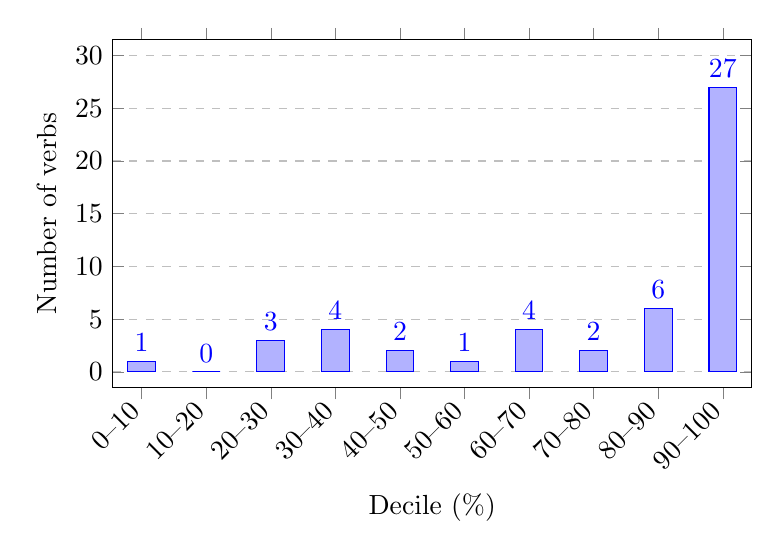
\begin{tikzpicture}
		\begin{axis}[
			ybar,
			bar width=10pt,
			enlargelimits=0.05,
			ylabel={Number of verbs},
			xlabel={Decile (\%)},
			symbolic x coords={0--10,10--20,20--30,30--40,40--50,50--60,60--70,70--80,80--90,90--100},
			xtick=data,
			xticklabel style={rotate=45, anchor=east},
			ymin=0,
			ymax=30,
			ytick={0,5,...,30},
			nodes near coords,
			width=0.8\textwidth,
			height=6cm,
			ymajorgrids=true,
			grid style={dashed,gray!50}
			]
			\addplot coordinates {
				(0--10,1) 
				(10--20,0) 
				(20--30,3) 
				(30--40,4) 
				(40--50,2)
				(50--60,1) 
				(60--70,4) 
				(70--80,2) 
				(80--90,6) 
				(90--100,27)
			};
		\end{axis}
	\end{tikzpicture}}
\end{figure}

\begin{figure}
	\caption{Decile distribution of the percentage of uninflected tokens of the infinitive in the periphrastic future construction for the 50 verbs of the sample}
	\label{09fig2}
	\scalebox{0.9}{
	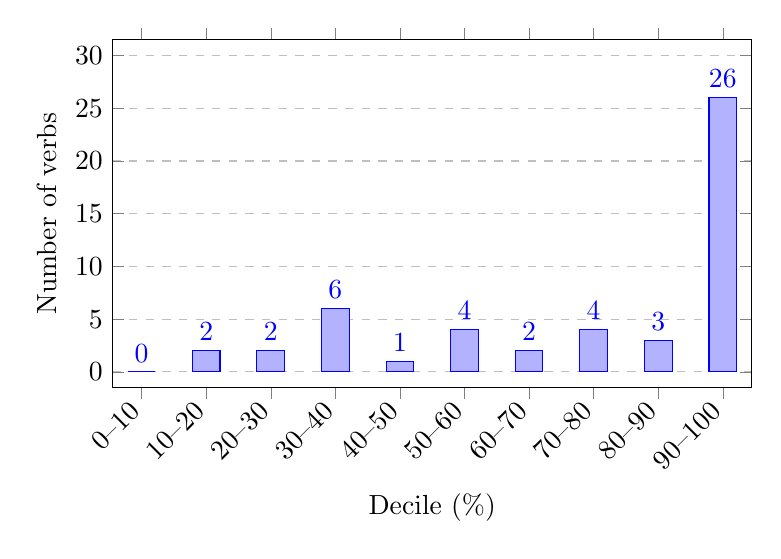
\begin{tikzpicture}
		\begin{axis}[
			ybar,
			bar width=10pt,
			enlargelimits=0.05,
			ylabel={Number of verbs},
			xlabel={Decile (\%)},
			symbolic x coords={0--10,10--20,20--30,30--40,40--50,50--60,60--70,70--80,80--90,90--100},
			xtick=data,
			xticklabel style={rotate=45, anchor=east},
			ymin=0,
			ymax=30,
			ytick={0,5,...,30},
			nodes near coords,
			width=0.8\textwidth,
			height=6cm,
			ymajorgrids=true,
			grid style={dashed,gray!50}
			]
			\addplot coordinates {
				(0--10,0) 
				(10--20,2) 
				(20--30,2) 
				(30--40,6) 
				(40--50,1)
				(50--60,4) 
				(60--70,2) 
				(70--80,4) 
				(80--90,3) 
				(90--100,26)
			};
		\end{axis}
	\end{tikzpicture}}
\end{figure}

The overall distribution trends are strikingly similar in the two datasets: the extreme lopsidedness to the right is highly remarkable and means that not only do the overwhelming majority of \ili{English}-origin verbs preferably appear in their uninflected guise in the two constructions, but more than half of them massively favor uninflectedness to the point that their inflected occurrences are almost negligible. This is a rather unexpected result given the extreme paucity of uninflected verbal forms in controlled written \ili{French}. At the individual level, almost all verbs are distributed in the same decile or in adjacent ones when comparing behavior in the two constructions, indicating that the ratio of uninflectedness is generally quite stable. The only exceptions are the verbs \emph{crush(er)}, \emph{switch(er)}, \emph{troll(er)}, and \emph{kick(er)}, and in all four cases it is the past participle form
that is markedly less inflected, suggesting that the dominance of uninflectedness may be slightly more advanced for the \emph{passé composé} construction.

The minority of verbs that are predominantly inflected are (in decreasing order of inflectedness): \emph{test(er)}, \emph{boost(er)},
\emph{shoot(er)}, \emph{bug(ger)}, \emph{boycott(er)}, \emph{clip(per)}, \emph{stop(per)}, \emph{tilt(er)}, \emph{tag(uer)}, \emph{perform(er)}, and \emph{kick(er)}. The main linguistic parameter which is hypothesized to markedly affect the distribution of uninflectedness is the relative establishment of the sampled verbs in the \ili{French} language. This parameter is operationalized here by the presence or absence of the \ili{English}-origin verb in a large recent \ili{French} dictionary of anglicisms\is{anglicism}, the \emph{Dictionnaire étymologique et critique des anglicismes}\is{anglicism} \citep{weisman2020}. Examination of the data is partially conclusive as the two overall distribution trends in Figures \ref{09fig3} and \ref{09fig4} are in stark contrast to each other. The dispersion of the dictionary-sanctioned verbs is quite high, indicating that the presence of a verb in the dictionary of anglicisms\is{anglicism} is not a reliable predictor of the ratio of uninflectedness, while the distribution of neologisms is extremely lopsided to the right, suggesting that novelty is correlated to a fairly large extent with massive uninflectedness. Among dictionary-sanctioned anglicisms\is{anglicism}, relative anteriority is not found to be a significant factor. In the set of nine \ili{English}-origin verbs that, according to \citet{weisman2020}, have been attested in \ili{French} for more than half a century, five --- \emph{test(er)}, \emph{boost(er)}, \emph{boycott(er)}, \emph{shoot(er)}, \emph{stop(per)} --- are predominantly inflected, but four --- \emph{drop(er)}, \emph{rush(er)}, \emph{switch(er)}, \emph{check(er)} --- are predominantly uninflected.

\begin{figure}[H]
	\caption{Decile distribution of the average percentage of uninflected tokens in the two constructions for the 16 dictionary-sanctioned verbs of the sample}
	\label{09fig3}
	\scalebox{0.9}{
	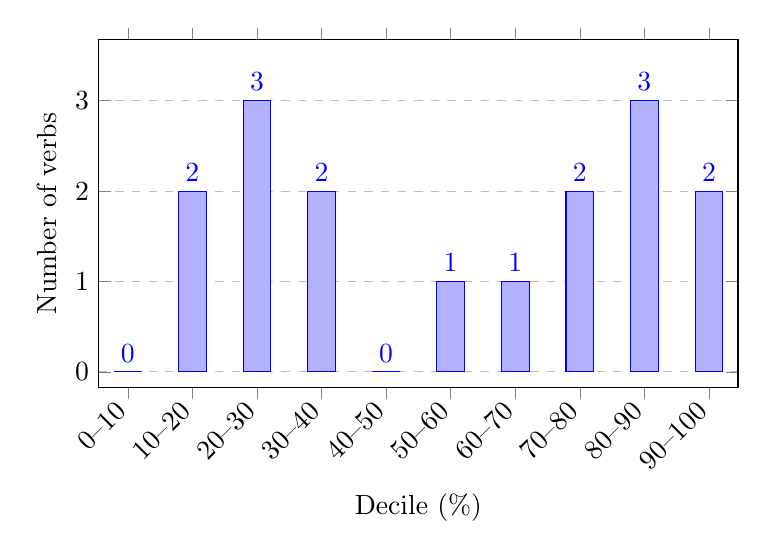
\begin{tikzpicture}
		\begin{axis}[
			ybar,
			bar width=10pt,
			enlargelimits=0.05,
			ylabel={Number of verbs},
			xlabel={Decile (\%)},
			symbolic x coords={0--10,10--20,20--30,30--40,40--50,50--60,60--70,70--80,80--90,90--100},
			xtick=data,
			xticklabel style={rotate=45, anchor=east},
			ymin=0,
			ymax=3.5,
			ytick={0,1,2,3},
			nodes near coords,
			width=0.8\textwidth,
			height=6cm,
			ymajorgrids=true,
			grid style={dashed,gray!50}
			]
			\addplot coordinates {
				(0--10,0) 
				(10--20,2) 
				(20--30,3) 
				(30--40,2) 
				(40--50,0)
				(50--60,1) 
				(60--70,1) 
				(70--80,2) 
				(80--90,3) 
				(90--100,2)
			};
		\end{axis}
	\end{tikzpicture}}
\end{figure}


\begin{figure}
	\caption{Decile distribution of the average percentage of uninflected tokens in the two constructions for the 34 neologisms of the sample}
	\label{09fig4}
	\scalebox{0.9}{
		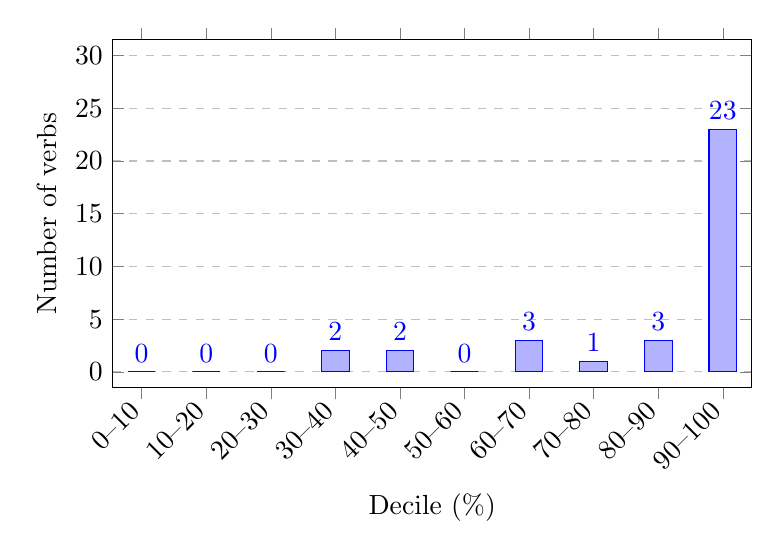
\begin{tikzpicture}
			\begin{axis}[
				ybar,
				bar width=10pt,
				enlargelimits=0.05,
				ylabel={Number of verbs},
				xlabel={Decile (\%)},
				symbolic x coords={0--10,10--20,20--30,30--40,40--50,50--60,60--70,70--80,80--90,90--100},
				xtick=data,
				xticklabel style={rotate=45, anchor=east},
				ymin=0,
				ymax=30,
				ytick={0,5,...,30},
				nodes near coords,
				width=0.8\textwidth,
				height=6cm,
				ymajorgrids=true,
				grid style={dashed,gray!50}
				]
				\addplot coordinates {
					(0--10,0) 
					(10--20,0) 
					(20--30,0) 
					(30--40,2) 
					(40--50,2)
					(50--60,0) 
					(60--70,3) 
					(70--80,1) 
					(80--90,3) 
					(90--100,23)
				};
			\end{axis}
		\end{tikzpicture}}
\end{figure}



\section{Discussion and conclusion} \label{09sec4}

The main finding of this exploratory study is that two verbal constructions of present-day \ili{French} massively display the nonstandard practice of dropping inflectional marking on the past participle and the infinitive in the context of written social media discourse\is{social media} and when the lexical verb is of \ili{English} origin. The choice of examining the \emph{passé composé} and the periphrastic future was initially guided by the intuition that inflection dropping seems to occur more frequently in these two constructions. This can be related to the fact that they correspond to doubly inflected composite verb forms (consisting of a lexical verb premodified by an auxiliary) while the other frequent finite forms of the \ili{French} verb (the \emph{présent}, the \emph{imparfait}, and the \emph{futur simple}) are simple verb forms which are singly inflected. Inflection dropping in simple verb forms is a less likely choice as it would lead to the loss of all morphological tense-aspect-mood (TAM) information. In contrast, in composite verb forms, dropping the inflectional marking on the lexical verb is not detrimental to the correct identification of the whole form and its TAM meaning. Inflection dropping should therefore be seen here as an unexpected and marked choice rather than an inconceivable one.

This view is also supported by the fact that verbal uninflectedness has been documented elsewhere in the periphery of the \ili{French} language. In their analysis of the outstanding grammatical features of the \emph{Multicultural Paris \ili{French}} (MPF) corpus, \citet{cappeaumoreno2017} point out that some groups of \ili{French} verbs appear under only one --- uninflected --- form. This notably applies to verbs originating from \emph{\isi{verlan}} (a \ili{French} argot based on syllable and phoneme reversal; cf. \citealt{mela1997}), as in (\ref{09ex5}--\ref{09ex7}), and from \ili{Romani}, as in (\ref{09ex8}--\ref{09ex9}):

\begin{exe}
	\ex \label{09ex5} J'ai envie d'\ul{sèpe}!
	\trans ‘I need to piss!’ \hfill \citep{tengour2024} \\
	(the inflected infinitive form \emph{séper} is expected; \emph{sèpe} is a verlanized\is{verlan} form of \emph{pisser})
	
	\ex J'ai \ul{vesqui} l'service militaire.
	\trans ‘I've skirted military service.’ \hfill \citep{tengour2024} \\
	(the inflected past participle form \emph{vesquié} is expected; \emph{vesqui} is a verlanized\is{verlan} form of \emph{esquiver})
	
	\ex \label{09ex7} C'est dead, Auxerre, ils m'ont \ul{tèj}.
	\trans ‘It's over, Auxerre have thrown me out.’ \hfill (Frantext)\nocite{frantext-noaccess}  \\
	(the inflected past participle form \emph{téjé} is expected; \emph{tèj} is a verlanized\is{verlan} form of \emph{jeter})
	
	\ex \label{09ex8} Comme dans les films qui collent des crampes au bide même quand on n'a rien \ul{bédave}.
	\trans ‘Like in the movies that give you stomach cramps even if you didn't smoke anything.’ \hfill (Frantext)\nocite{frantext-noaccess} \\
	(the inflected past participle form \emph{bédavé} is expected)
	
	\ex \label{09ex9} Peur ! Peur ! Quand tu dois \ul{poucave} ton pote...
	\trans ‘Fear! Fear! When you have to snitch on your buddy...’ \hfill (Frantext)\nocite{frantext-noaccess}  \\
	(the inflected infinitive form \emph{poucaver} is expected)
\end{exe}

Verbal uninflectedness has also been documented to appear when \ili{French} has been in intense contact with \ili{English}. \citet{duboissankoff1997} report that, in Louisiana \ili{French}, \ili{English}-origin verbs are typically adapted to the \ili{French} morphological system, except for the past participle and infinitive forms, for which the bare stem is used, as illustrated in (\ref{09ex10}--\ref{09ex11}), and they conclude that such verbs can be seen as belonging to a distinct \isi{conjugation class}:

\begin{exe}
	\ex \label{09ex10} Tu crois que noncle Pierre a \ul{enjoy} sa visite ?
	\trans ‘Do you think that Uncle Pierre enjoyed his visit?’ \\
	(the inflected past participle form \emph{enjoyé} is expected)
	
	\ex \label{09ex11} Je crois ici là on peut mieux \ul{discipline} notre enfant.\footnote{It is unclear why the form ``\emph{discipline}" (which is the only infinitive form given by the authors as an illustrative example) is considered to be an \ili{English}-origin verb. In a form of circular reasoning, it may be that its uninflectedness is seen as a justification for its status as an anglicism\is{anglicism}. Other illustrative evidence can be adduced, such as \emph{ça va flood cette section là} `they're going to flood this section', or \emph{je vas le back sûr} `I'll definitely back him' \citep[19, 26]{root2018}.}
	\trans ‘I think that here we can better discipline our kid.’ \\
	(the inflected infinitive form \emph{discipliner} is expected)
\end{exe}

In an experimental study of the conditions influencing morphological (non\mbox{-})in\-tegration, \citet{root2018} offers a nuanced and quantitatively driven examination of the phenomenon, positing the existence of a class of loan-verbs characterized by variable integration, for which some slots of the verbal paradigm are preferentially filled with bare forms and others with morphologically integrated ones. This hypothesis is partially supported by his data since inflected forms account for 50\% of the tokens for the conditional, for 32\% for the \emph{imparfait}, for 17\% for the past participle, and for 13\% for the infinitive.

A similar situation is found in some \ili{French}-based hybrid urban vernaculars of western Africa. In \ili{Nouchi}, a hybrid language of Côte d'Ivoire mixing \ili{French} with other European languages and several Niger-Congo languages \citep{sande2015, boutin2021}, \ili{French}-origin verbs in \emph{passé composé} and periphrastic future constructions are inflected in the same way as in Standard \ili{French} while verbs of other origins (e.g. Dyula, Malinke, or \ili{English}) remain uninflected \citep{ahua2008, atsencho2014}. Similarly, in \ili{Camfranglais}, a hybrid language of Cameroon mixing \ili{French}, \ili{English}, Cameroonian Pidgin \ili{English}, and a number of Cameroonian languages \citep{kiesling2022}, verbs of non-\ili{French} origin are uninflected in the \emph{passé composé} and periphrastic future constructions, as in \citeauthor{bogni2018}'s (\citeyear[185]{bogni2018}) examples in (\ref{09ex12}--\ref{09ex13}):

\begin{exe}
	\ex \label{09ex12} J'ai \ul{begin} à \ul{play} les cartes frons.
	\trans ‘I've been playing cards for a long time.’ \\
	(the inflected past participle form \emph{beginé} and the inflected infinitive form \emph{player} are expected)
	
	\ex \label{09ex13} Nous allons \ul{back} autour de 17 heures.
	\trans ‘We'll get back around 5 p.m.’ \\
	(the inflected infinitive form \emph{backer} is expected)
\end{exe}

Like Dubois and Sankoff for Louisiana \ili{French}, \citet{bogni2018} concludes that verbs of non-\ili{French} origin form a distinct (``fourth group") \isi{conjugation class} in \ili{Camfranglais}. In line with Root's quantitative approach for Louisiana \ili{French}, \citeauthor{nchare2010}'s (\citeyear{nchare2010}) analysis of a large dataset of online \ili{Camfranglais} interactions provides a slightly nuanced picture of language in use and confirms a particularly pronounced tendency towards uninflectedness, with 98\% of bare past participles, 91\% of bare infinitives, and a morphological class of exceptions that reportedly comprises all denominal verbs.

This brief overview of similar phenomena in a variety of language-contact settings demonstrates that the massive Twitter-wide uninflectedness of many \ili{French} verb forms of \ili{English} origin, while unexpected because it violates a presumably categorical norm, may not, after informed consideration, be truly exceptional. It also suggests that unadapted forms are not only a marked choice flagging foreignness and peripherality, but also, in some cases, markers of in-group membership that may contribute to the characterization of a sociolect --- here, that of (young) tweeters and, more generally, that of (young) KSC users\is{keyboard-to-screen communication (KSC)}.

An obvious limitation of this exploratory investigation is that the analysis is blind to the geographic and demographic distribution of the collected data. Regarding the former dimension, it can be hypothesized that European, North American, and African varieties of \ili{French} accommodate uninflectedness in fairly similar ways, but this assumption will need to be empirically confirmed in future research. Regarding the latter dimension, \citet{bouchard2023} has found a highly significant correlation between age and the reported use of morphologically unintegrated \ili{English}-origin verbs in Quebec \ili{French}, with younger people much more likely to use such forms, and her findings are likely to generalize across varieties of present-day \ili{French}. It also remains to be seen whether uninflectedness is becoming more prevalent, or will soon extend, in a quantitatively significant way beyond \ili{English}-origin verbs, i.e. to the native lexicon. \citet[79]{cappeaumoreno2017} and \citet[737]{gadethambye2018} report various cases of inflection dropping in non-\ili{English} and cognate verbs in the MPF corpus, as illustrated in (\ref{09ex14}--\ref{09ex17}):

\begin{exe}
	\ex \label{09ex14} On s'est fait \ul{carotte} en fait.
	\trans ‘We've actually been screwed.’ \\
	(the inflected infinitive form \emph{carotter} is expected)
	
	\ex \label{09ex15} Les gens quand ils sont asthmatiques ils leur donnent de l'air pas à \ul{graille}.
	\trans ‘When people have asthma, they're given some air, not something to eat.’ \\
	(the inflected infinitive form \emph{grailler} is expected)
	
	\ex \label{09ex16} Je vais pas te \ul{mytho}.
	\trans ‘I'm not gonna lie to you.’ \\
	(the inflected infinitive form \emph{mythonner} is expected)
	
	\ex \label{09ex17} Je me fais \ul{contrôle}.
	\trans ‘I had my ticket checked.’ \\
	(the inflected infinitive form \emph{contrôler} is expected)
\end{exe}

It therefore cannot be ruled out that, in the course of a generation, uninflectedness in a number of verbal constructions will have become a hallmark feature of colloquial \ili{French}.
 
%\section*{Abbreviations}
%\begin{tabularx}{.45\textwidth}{lQ}
%... & \\
%... & \\
%\end{tabularx}
%\begin{tabularx}{.45\textwidth}{lQ}
%... & \\
%... & \\
%\end{tabularx}

\section*{Acknowledgements}
Earlier versions of this research have been presented to several academic audiences and we are grateful for the many comments and suggestions we have received. We also duly thank Bruno Courbon, Sophie Kraeber, and two anonymous reviewers for their very valuable feedback on the first draft of this article. The usual disclaimers apply.

%\section*{Contributions}
%John Doe contributed to conceptualization, methodology, and validation.
%Jane Doe contributed to writing of the original draft, review, and editing.


{\sloppy\printbibliography[heading=subbibliography,notkeyword=this]}
\end{document}
